\documentclass[compress]{beamer}
\mode<presentation>
{
 \usetheme{Vilanova}
}

\usepackage[english]{babel}

\usepackage[latin1]{inputenc}

\usepackage{times}
\usepackage[T1]{fontenc}

\usepackage{amsfonts}
\usepackage{amsmath}
\usepackage{amssymb}
\usepackage{tikz}
%\usepackage{url}


\title{Image geometry in ORFEO Toolbox}

\subtitle
{Sensor models and map projections} % (optional)


\author
{J. Inglada\inst{1} , E. Christophe\inst{2}}
\normalsize

\institute[Cnes, Crisp] % (optional, but mostly needed)
{\inst{1}\textsc{Centre d'�tudes Spatiales de la Biosph�re, Toulouse, France}
\and
\inst{2}\textsc{Centre for Remote Imaging, Sensing and Processing,\\ National University of Singapore}
}

\date{}

\subject{Image geometry in ORFEO Toolbox}


\pgfdeclareimage[height=96mm,width=128mm]{background}{fondsClairSansLogo}
\setbeamertemplate{background}{\pgfuseimage{background}}
\pgfdeclareimage[height=0.6cm]{logoIncrust}{logoIncrust}
\pgfdeclareimage[height=0.5cm]{logo_cesbio}{logo_cesbio}
\pgfdeclareimage[height=0.35cm]{logo_crisp}{logo_crisp}
\logo{
\begin{tabular}{lp{0.10\textwidth}lp{0.25\textwidth}r}
\href{http://www.cesbio.ups-tlse.fr/}{\pgfuseimage{logo_cesbio}}\href{http://www.crisp.nus.edu.sg/}{\pgfuseimage{logo_crisp}}
&&\footnotesize{IGARSS 2010, Honolulu}&&
\href{http://www.orfeo-toolbox.org}{\pgfuseimage{logoIncrust}}\\
\end{tabular}
}



% Delete this, if you do not want the table of contents to pop up at
% the beginning of each subsection:
\AtBeginSubsection[]
{
  \begin{frame}<beamer>
    \frametitle{Outline}
    \tableofcontents[currentsection,currentsubsection]
  \end{frame}
}




% If you wish to uncover everything in a step-wise fashion, uncomment
% the following command: 

%\beamerdefaultoverlayspecification{<+->}

\begin{document}

\begin{frame}
  \titlepage
{\tiny This content is provided under a Creative Commons
  Attribution 3.0 Unported License} \href{http://creativecommons.org/licenses/by/3.0/}{
\includegraphics[width=0.05\textwidth]{../Ressources/CC-licence.png}}
\end{frame}

\section*{Introduction}

\begin{frame}

  \frametitle{Introduction}
  \hspace*{-1cm}
  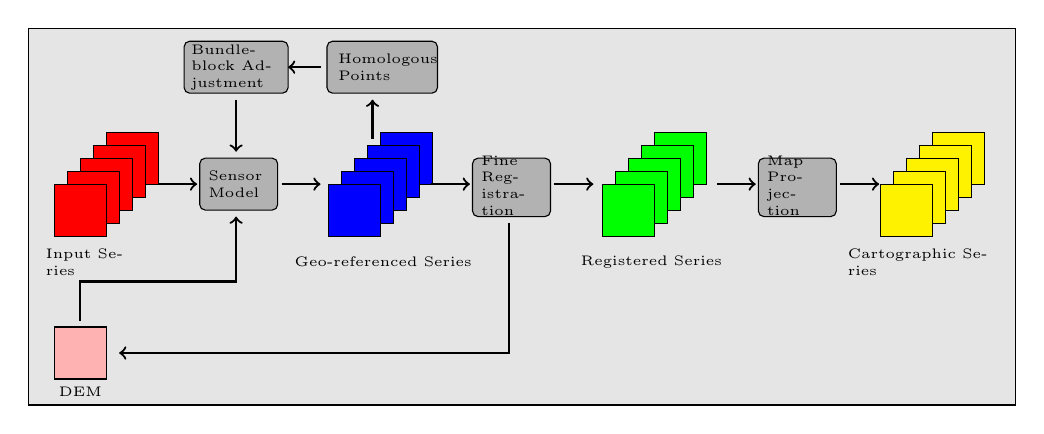
\begin{tikzpicture}[scale=0.165]
    \tiny
    \draw[fill=black!10] (-1,-12) rectangle (75,17);
     \foreach \x in {5,...,1}
       \draw[fill=red] (\x,\x) rectangle +(4,4);
     \node[fill=black!10, text width= 1.2cm] (InputSeries) at
       (4,-1) {Input Series};
     \pause
     \draw[->,thick] (9,5) --  +(3,0);
     \pause
     \draw[fill=black!30,rounded corners=2pt] (12.2,3) rectangle +(6,4);
     \node[text width= 0.7cm] (SensorModel) at (15,5) {Sensor Model};
     \pause
     \draw[fill=red!30] (1,-10) rectangle +(4,4);
     \node[fill=black!10, text width= 1.2cm] (DEM) at
       (5,-11) {DEM};
     \pause
     \draw[->,thick] (3,-5.5) --  ++(0,3) -- ++(12,0) -- ++(0,5);
     \pause
     \draw[->,thick] (18.5,5) --  +(3,0);
     \pause
     \foreach \x in {5,...,1}
       \draw[fill=blue,xshift=600pt] (\x,\x) rectangle +(4,4);
     \node[fill=black!10, text width= 2.8cm] (GeoRefSeries) at
       (28,-1) {Geo-referenced Series};
\pause
      

       \draw[->,thick] (25.5,8.5) --  +(0,3);
       
     \draw[fill=black!30,rounded corners=2pt] (22,12) rectangle +(8.5,4);
     \node[text width= 0.7cm] (HomPoExtr) at (25,14) {Homologous
     Points};

     \draw[->,thick] (21.5,14) --  +(-2.5,0);

     \draw[fill=black!30,rounded corners=2pt] (11,12) rectangle +(8,4);
     \node[text width= 1.3cm] (BBAdj) at (15.5,14) {Bundle-block
     Adjustment};

     \draw[->,thick] (15,11.5) --  +(0,-4);

     \pause
      \draw[->,thick] (30,5) --  +(3,0);
      \pause
     \draw[fill=black!30,rounded corners=2pt] (33.2,2.5) rectangle +(6,4.5);
     \node[text width= 0.7cm] (FineRegistration) at (36,4.9) {Fine
     Registration};
     \pause

     
     \draw[->,thick] (39.5,5) --  +(3,0);
     \pause
     \foreach \x in {5,...,1}
       \draw[fill=green,xshift=1200pt] (\x,\x) rectangle +(4,4);
     \node[fill=black!10, text width= 1.8cm] (RegistSeries) at
       (47,-1) {Registered Series};
     \pause
     \draw[->,thick] (36,2) --  ++(0,-10) -- ++(-30,0);

     \pause
      \draw[->,thick] (52,5) --  +(3,0);
      \pause
     \draw[fill=black!30,rounded corners=2pt] (55.2,2.5) rectangle +(6,4.5);
     \node[text width= 0.7cm] (CartoProjection) at (58,4.9) {Map Projection};
     \pause

     
     \draw[->,thick] (61.5,5) --  +(3,0);
     \pause
     \foreach \x in {5,...,1}
       \draw[fill=yellow,xshift=1810pt] (\x,\x) rectangle +(4,4);
     \node[fill=black!10, text width= 1.95cm] (CartoSeries) at
       (68,-1) {Cartographic Series};
     
       
  \end{tikzpicture}
\end{frame}

%% \begin{frame}
%%   \frametitle{Introduction}
%%  \begin{block}{How to register image series}
%%  \begin{itemize}
%%  \item Sensor models and bundle-block adjustment
%%  \item Homologous point extraction
%%  \item Fine registration
%%  \end{itemize}
%%  \end{block}
%%  \begin{block}{How to measure the quality}
%%  \begin{itemize}
%%  \item Choosing the reference
%%  \item Quality measures
%%  \end{itemize}
%%  \end{block}
%%  \end{frame}

\begin{frame}
  \frametitle{Outline of the presentation}
  \tableofcontents[pausesections]
  % You might wish to add the option [pausesections]
\end{frame}

\section[Models]{Sensor models}


\begin{frame}
  \frametitle{Sensor models}

  \framesubtitle{What is a sensor model}
Gives the relationship between image $(l,c)$ and ground $(X,Y)$ coordinates for every
pixel in the image.
\pause
\begin{displaymath}
  \begin{array}{cc}
    Forward & \\
    X = f_x(l,c,h,\vec\theta) & Y = f_y(l,c,h,\vec\theta)\\
     & \\ \pause
    Inverse & \\
    l = g_l(X,Y,h,\vec\theta) & c = g_c(X,Y,h,\vec\theta)
  \end{array}
\end{displaymath}
\pause
Where $\vec\theta$ is the set of parameters which describe the sensor
and the acquisition geometry.\\
\pause
Height (DEM) must be known.
  
\end{frame}

\begin{frame}
  \frametitle{Sensor models}

  \framesubtitle{Types of sensor models}
  \begin{itemize}
    \item Physical models
      \begin{itemize}
	\item Rigorous, complex, highly non-linear equations of the
	sensor geometry.
	\item Usually, difficult to invert.
	\item Parameters have a physical meaning.
	\item Specific to each sensor.
      \end{itemize}
    \item General analytical models
      \begin{itemize}
	\item Ex: polynomial, rational functions, etc.
	\item Less accurate.
	\item Easier to use.
	\item Parameters may have no physical meaning.
      \end{itemize}
  \end{itemize}

\end{frame}

\begin{frame}
  \frametitle{Sensor models}

  \framesubtitle{OTB's Approach}
  \begin{itemize}
    \item Use factories: models are automatically generated using
    image meta-data.
    \item Currently tested models:
      \begin{itemize}
	\item RPC models: Quickbird, Ikonos
	\item Physical models: SPOT5
	\item SAR models: ERS, ASAR, Radarsat, Cosmo, TerraSAR-X, Palsar
      \end{itemize}
    \item Under development:
      \begin{itemize}
        \item Formosat, WorldView 2
      \end{itemize}      
  \end{itemize}
\end{frame}


\begin{frame}
\frametitle{Hands On}
\begin{enumerate}
\item Monteverdi: Open a Quickbird image in sensor geometry
\item Display the image
\item Observe how the geographic coordinates are computed when the cursor
      moves around the image
\end{enumerate}
\end{frame}

\begin{frame}
  \frametitle{Sensor models}

  \framesubtitle{How to use them: ortho-registration}
  \begin{enumerate}
    \item Read image meta-data and instantiate the model with the
    given parameters.
  \item Define the ROI in ground coordinates (this is your output
  pixel array)
  \item Iterate through the pixels of coordinates $(X,Y)$:
    \begin{enumerate}
      \item Get $h$ from the DEM
      \item Compute $(c,l) = G(X,Y,h,\vec\theta)$
      \item Interpolate pixel values if $(c,l)$ are not grid coordinates.
    \end{enumerate}
  \end{enumerate}
\end{frame}

\begin{frame}
\frametitle{Hands On}
\begin{enumerate}
\item Monteverdi: Geometry $\rightarrow$ Orthorectification
\item Select the image to orthorectify
\item Set the parameters
\item Save the result
\item Repeat for the other image with the same parameters
\item Display the two images together
\end{enumerate}
\end{frame}


\begin{frame}
  \frametitle{Sensor models}
  \framesubtitle{Limits of the approach}

  \begin{itemize}
    \item Accurate geo-referencing needs:
      \begin{itemize}
	\item Accurate DEM
	\item Accurate sensor parameters, $\vec\theta$
      \end{itemize}
    \item For time image series we need \alert{accurate co-registration}:
      \begin{itemize}
      \item Sub-pixel accuracy
      \item For every pixel in the scene
      \end{itemize}
    \item Current DEM's and sensor parameters can not give this
    accuracy.
    \item Solution: use redundant information in the image series!
  \end{itemize}
\end{frame}

\section{Optimizations}
\subsection[BBA]{Bundle-block adjustment}

\begin{frame}
  \frametitle{Bundle-block adjustment}
  \framesubtitle{Problem position}
  \begin{columns}[T]
\column{.5\textwidth}
  \begin{itemize}
    \item The image series is geo-referenced (using the available DEM,
    and the prior sensor parameters).
    \item We assume that homologous points (GCPs, etc.) can be easily
    obtained from the geo-referenced series : $HP_i = (X_i,Y_i,h_i)$
    \item For each image, and each point, we can write:
    $(l_{ij},c_{ij}) = G_j(X_i,Y_i,h_i,\vec\theta_j)$
  \end{itemize}
\column{.5\textwidth}
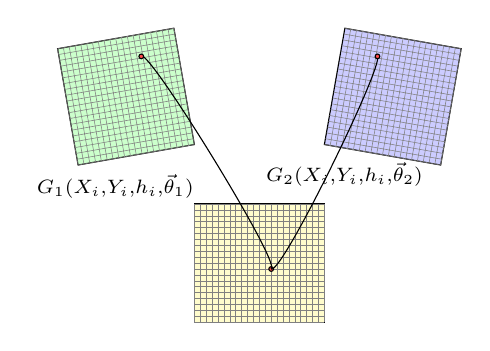
\begin{tikzpicture}[scale=0.15]
\draw[fill=yellow!20] (-5.5,-15.5) rectangle (5.5,-5.5);
    \draw[step=0.5, gray, very thin] (-5.5,-15.5) grid (5.5,-5.5);

    \draw[fill=green!20,rotate=10] (-15.5,0.5) rectangle (-5.5,10.5);
    \draw[step=0.5, gray, very thin,rotate=10] (-15.5,0.5) grid
    (-5.5,10.5);

    \draw[fill=blue!20,rotate=-10] (5.5,0.5) rectangle (15.5,10.5);
    \draw[step=0.5, gray, very thin,rotate=-10] (5.5,0.5) grid
    (15.5,10.5);

    \pause
    \draw[fill=red!70] (1,-11) circle (0.2);
    \pause
    \draw (1,-11) .. controls +(30:1cm) and +(60:1cm) .. (-10,7);
    \pause
    \draw[fill=red!70] (-10,7) circle (0.2);
    \pause
    \node (eq1) at (-12.2,-4) {$\scriptstyle{G_1(X_i,Y_i,h_i,\vec\theta_1)}$};
    \pause
    \draw (1,-11) .. controls +(-30:1cm) and +(-60:1cm) .. (10,7);
    \pause
    \draw[fill=red!70] (10,7) circle (0.2);
    \pause
    \node (eq2) at (7.2,-3) {$\scriptstyle{G_2(X_i,Y_i,h_i,\vec\theta_2)}$};
    
\end{tikzpicture}
\begin{itemize}
      \item Everything is known.
\end{itemize}
  \end{columns}
\end{frame}

\begin{frame}
  \frametitle{Bundle-block adjustment}
  \framesubtitle{Model refinement}
  \begin{itemize}
    \item If we define $\vec\theta_j^R = \vec\theta_j +
    \vec{\Delta\theta_j}$ as the refined parameters,
    $\vec{\Delta\theta_j}$ are the unknowns of the model refinement
    problem.
    \item We have much more equations than unknowns if enough HPs are
    found.
    \item We solve using non-linear least squares estimation.
      \begin{itemize}
	\item The derivatives of the sensor model with respect to its
	parameters are needed.
      \end{itemize}
  \end{itemize}
  
\end{frame}

\begin{frame}
  \frametitle{Hands On}
  \framesubtitle{Manually register 2 images}
\vspace*{-0.6cm}
\small
  \begin{itemize}
  \item Monteverdi: Geometry $\rightarrow$ Homologous points extraction
  \item Select 2 images with a common region
  \item The GUI lets you select a transformation
  \item You can select homologous points in the zoom images and add
    them to the list
  \item When several homologous points are available, you can evaluate
    the transform
  \item Once the transform is evaluated, you can use the {\em guess}
    button to predict the position in the moving image of a point
    selected in the fixed image
  \item The GUI displays the parameters of the transform estimated as
    well as individual error for each point and the MSE
  \item You can remove from the list the points with higher error
  \end{itemize}
\end{frame}

%
%\begin{frame}
%\frametitle{Homologous point extraction}
%\framesubtitle{From manual to automatic procedures}
%\begin{itemize}
%  \item Manual extraction can be used for a few images and for a few
%  points
%  \item We are interested in many images (long time series) and many
%  points (in order to reduce registration errors)
%  \item Proposed procedure
%    \begin{enumerate}
%      \item Choose candidate points
%      \item Define a similarity measure
%      \item Optimize the measure
%    \end{enumerate}
%\end{itemize}
%
%\end{frame}
%
%\begin{frame}
%  \frametitle{Salient points}
%  \begin{itemize}
%    \item Points where the image information content is high
%    \item Corners, segment extremities, etc.
%    \item Harris detector: $det(\mu) - \alpha trace^2(\mu)$ with\pause
%    \begin{displaymath}
%    \mu(\mathbf{x},\sigma_I,\sigma_D) = \sigma_D^2 g(\sigma_I)\star
%    \left[\begin{array}{cc} L_x^2(\mathbf{x},\sigma_D) &
%    L_xL_y(\mathbf{x},\sigma_D)\\ L_xL_y(\mathbf{x},\sigma_D)&
%    L_y^2(\mathbf{x},\sigma_D) \end{array}\right]\end{displaymath}
%    \pause
%  \begin{center}
%      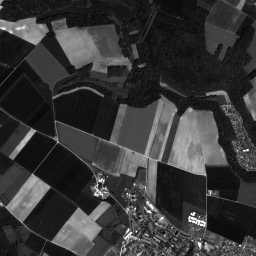
\includegraphics[width=0.3\textwidth]{ROISpot5.png}
%      \pause
%      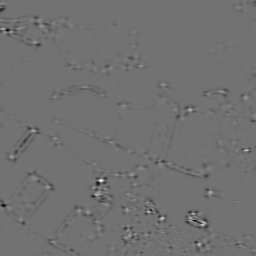
\includegraphics[width=0.3\textwidth]{ROISpot5Harris.png}
%  \end{center}    
%  \end{itemize}
%
%\end{frame}
%
%\begin{frame}
%  \frametitle{Similarity measures}
%  \framesubtitle{Definition}
%  \begin{itemize}
%    \item Let $I$ and $J$ be 2 images and let $c$ be a similarity criterion,
%    a similarity measure $S = f(I,J,c)$ has a global maximum when $I$ are $J$
%    identical with respect to $c$.
%  \item Problem: find $f$ which efficiently exploits $c$.
%  \item Problem bis: $f$ has to be easily and robustly estimated ...
%  \item Examples: L-2 norm, correlation coefficient, etc.
%  \end{itemize}
%\end{frame}
%



%\begin{frame}
%  \frametitle{Optimization}
%  \begin{itemize}
%    \item So the problem is:
%      \begin{itemize}
%	\item For each candidate point, find $(\Delta_x,\Delta_y)$
%	maximizing the similarity.
%      \end{itemize}
%    \item For integer pixel precision:
%      \begin{itemize}
%	\item Exhaustive search
%      \end{itemize}
%    \item For sub-pixel precision:
%      \begin{itemize}
%	\item Smart optimization
%	\item Image interpolation
%      \end{itemize}
%  \end{itemize}
%\end{frame}
%

\subsection{Fine registration}
\begin{frame}
\frametitle{Why fine registration?}
\begin{itemize}
  \item Homologous points have been used to refine the sensor model
  \item Residual misregistrations exist because of:
    \begin{itemize}
      \item DEM errors
      \item Sensor model approximations
      \item Surface objects (high resolution imagery)
    \end{itemize}
  \item We want to find the homologous point
    \begin{itemize}
      \item of every pixel in the reference image
      \item with sub-pixel accuracy
    \end{itemize}
  \item This is called \alert{disparity map}
\end{itemize}
\end{frame}

\begin{frame}
  \frametitle{Fine registration (under development)}
  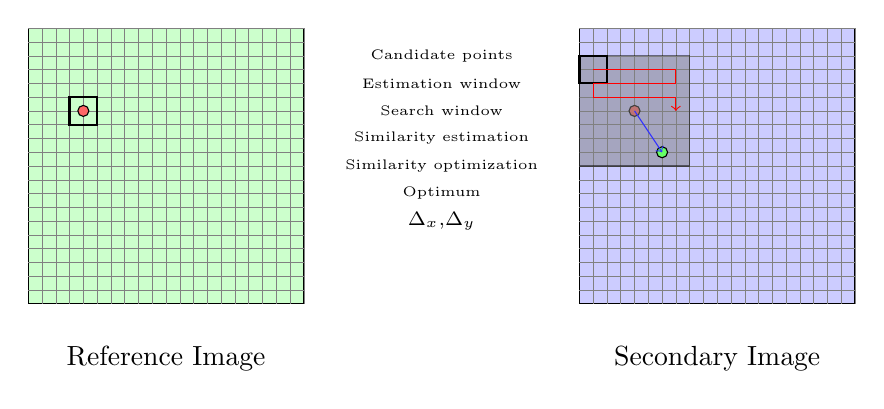
\begin{tikzpicture}[scale=0.35]
    \draw[fill=green!20] (5,5) rectangle (15,15);
    \draw[step=0.5, gray, very thin] (5,5) grid (15,15);
    \node (Reference) at (10,3) {Reference Image};

    \draw[fill=blue!20] (25,5) rectangle (35,15);
    \draw[step=0.5, gray, very thin] (25,5) grid (35,15);
    \node (Reference) at (30,3) {Secondary Image};
    \pause
    \draw[fill=red!60] (7,12) circle (0.2);
    \draw[fill=red!60] (27,12) circle (0.2);
    \node (CPs) at (20,14) {\tiny Candidate points};
    \pause
    \draw[thick] (6.5,11.5) rectangle +(1,1);
    \node (EW) at (20,13) {\tiny Estimation window};
    \pause
    \draw[fill=gray, opacity=0.5] (25,10) rectangle +(4,4);
    \node (SW) at (20,12) {\tiny Search window};
    \pause
    \draw[thick] (25,13) rectangle +(1,1);
    \node (SEW) at (20,11) {\tiny Similarity estimation};
    \pause
    \draw[red,->] (25.5,13.5) --  ++(3,0) -- ++(0,-0.5) -- ++(-3,0) -- ++(0,-0.5) --++(3,0) -- ++(0,-0.5)  ;
    \node (OPT) at (20,10) {\tiny Similarity optimization};
    \pause
    \draw[fill=green!60] (28,10.5) circle (0.2);
    \node (OPTF) at (20,9) {\tiny Optimum};
    \pause
    \draw[blue!80,->] (27,12) -- (28,10.5);
    \node (Deltas) at (20,8) {$\scriptstyle{\Delta_x,\Delta_y}$};
    
  \end{tikzpicture}
  \end{frame}


% \begin{frame}
%   \frametitle{Disparity maps}
%   \framesubtitle{Input data}
%   \begin{center}
%     \begin{tikzpicture}
%       \node (RefIm) at (0,0)
%       {\includegraphics[width=0.3\textwidth]{/home/inglada/rapports/Presentations/Bolzano/Images/spotb3}};
%       \node (RefImText) at (0,-2) {Reference Image};
%       \node (SecIm) at (4,0)
%       {\includegraphics[width=0.3\textwidth]{/home/inglada/rapports/Presentations/Bolzano/Images/ERS}};
%       \node (SecImText) at (4,-2) {Secondary Image};
%       \node (MNT) at (8,0)
%       {\includegraphics[width=0.3\textwidth]{/home/inglada/rapports/Presentations/Bolzano/Images/mnt_final.pdf}};
%       \node (MNTText) at (8,-2) {DEM};
%     \end{tikzpicture}
  
%   \end{center}
%   \end{frame}

%   \begin{frame}
%   \frametitle{Disparity maps}
%   \framesubtitle{Estimation results}
%   \begin{center}
%     \begin{tikzpicture}
%       \node (DecLig) at (0,0)
%       {\includegraphics[width=0.3\textwidth]{/home/inglada/rapports/Presentations/Bolzano/Images/dec_lig.pdf}};
%       \node (DecLigText) at (0,-2) {$\Delta_y$ Image};
%       \node (DecCol) at (4,0)
%       {\includegraphics[width=0.3\textwidth]{/home/inglada/rapports/Presentations/Bolzano/Images/dec_col.pdf}};
%       \node (DecColText) at (4,-2) {$\Delta_x$ Image};
%       \node (MNT) at (8,0)
%       {\includegraphics[width=0.3\textwidth]{/home/inglada/rapports/Presentations/Bolzano/Images/mnt_final.pdf}};
%       \node (MNTText) at (8,-2) {DEM};
%     \end{tikzpicture}
  
%   \end{center}

% \end{frame}

%   \begin{frame}
%   \frametitle{Disparity maps}
%   \framesubtitle{Critical parameters}

%   \begin{itemize}
%     \item Estimation window: determines the disparity map spatial
%     resolution
%     \begin{itemize}
%       \item Trade-off between resolution and robust estimation
%     \end{itemize}
%     \item Search window
%       \begin{itemize}
% 	\item Trade-off between large excursions and false matchings
%       \end{itemize}
%     \item Interpolation filter
%       \begin{itemize}
% 	\item Trade-off between speed and artifacts (see later)
%       \end{itemize}
%   \end{itemize}
  
%   \end{frame}

% \begin{frame}
%   \frametitle{Interpolation artifacts}
%   \framesubtitle{Observed behaviour}

%     \begin{center}
%     \begin{tikzpicture}
%       \node (Histocol) at (0,0)
%       {\includegraphics[width=0.5\textwidth]{/home/inglada/rapports/Presentations/Bolzano/Images/histosGrillesERSSPOTCol.pdf}};
%       %\node (HistoColText) at (0,-2.5) {$\Delta_y$ histogram};
%       \node (HistoLig) at (5.5,0)
%       {\includegraphics[width=0.5\textwidth]{/home/inglada/rapports/Presentations/Bolzano/Images/histosGrillesERSSPOTLig.pdf}};
%       %\node (HistoLigText) at (5.5,-2.5) {$\Delta_x$ histogram};
%     \end{tikzpicture}
  
%   \end{center}
%     \pause
%     \begin{itemize}
%       \item Wrong shifts are measured for $k\times\frac{1}{2}$ pixel
%       positions
%       \begin{itemize}
% 	\item When the noisy image is interpolated!
%       \end{itemize}
%     \end{itemize}

% \end{frame}

% \begin{frame}
%   \frametitle{Interpolation artifacts}
%   \framesubtitle{Explanation \& solution}
%   \begin{itemize}
%     \item The interpolators have a smoothing effect which depends on
%     the interpolated shift
%     \begin{tikzpicture}
%       \node (Linear) at (0,0)
%       {\includegraphics[width=0.5\textwidth]{/home/inglada/rapports/Presentations/Bolzano/Images/linear.pdf}};
%       \node (Spline) at (5.5,0)
%       {\includegraphics[width=0.5\textwidth]{/home/inglada/rapports/Presentations/Bolzano/Images/spline.pdf}};
%     \end{tikzpicture}  
%     \item Use good interpolators
%     \item Low-pass filter your images
%       \end{itemize}


%   \end{frame}

% \begin{frame}
%   \frametitle{Similarity measures}
%   \framesubtitle{The multi-sensor case}
%   \begin{itemize}
%     \item The correlation surface
%       \begin{displaymath}
% 	\rho_{I,J}(\Delta x, \Delta y) = \frac{\int\int I(x,y)J(x+\Delta x,
% y+\Delta y) dx dy}{\sqrt{\int\int I(x,y) dx dy \int\int J(x+\Delta x,
% y+\Delta y) dx dy}}
%       \end{displaymath}
%      \item Is the correlation coefficient between image patches
%        \begin{displaymath}
% 	 \rho(I,J) = \frac{1}{N}\frac{\sum_{x,y}(I(x,y)-m_I)(J(x,y)-m_J)}{\sigma_I
% \sigma_J}
%        \end{displaymath}
%        \item Drawbacks:
% 	 \begin{itemize}
% 	   \item Only a linear relationship between intensities can be measured:
% $j = \alpha i + \beta$
% \item Not usable for the general multi-sensor case
% 	 \end{itemize}
%   \end{itemize}

% \end{frame}

% \begin{frame}
%   \frametitle{Similarity measures}
%   \framesubtitle{The multi-sensor case}
%   \begin{itemize}
%     \item Probabilistic interpretation of the correlation:
%       \begin{displaymath}
% 	\rho(I,J) = \sum_{(i,j)}\frac{(i-m_I)(j-m_J)}{\sigma_I
% \sigma_J}p_{ij}
%       \end{displaymath}
%       where $p_{ij}$ is the joint probability of intensities $i$ and
%       $j$ appearing on homologous pixels
%     \item So we are measuring the likelihood of the following (linear) model:
%     \begin{displaymath}
%       j = (i-m_I)\frac{\sigma_J}{\sigma_I}+m_J
%     \end{displaymath}
%   \end{itemize}
% \end{frame}

% \begin{frame}
%   \frametitle{Similarity measures}
%   \framesubtitle{The multi-sensor case}
%   \begin{itemize}
%   \item Other models can be evaluated
%     \begin{itemize}
%       \item Linear $L_n(I,J) = \sum_{i,j} \left| i - j\right|^n p_{ij}$
%       \item Diagonal moment: $MD(I,J) = \sum_{i,j}\left| i - j\right|(i+j-\sigma_1-\sigma_2) p_{ij}$
%       \item Cluster Shade: $C_{shade}(I,J) = \sum_{i,j} (i+j-\sigma_1-\sigma_2)^3 p_{ij}$
%       \item Cluster Prominence: $C_{pro}(I,J) = \sum_{i,j} (i+j-\sigma_1-\sigma_2)^4 p_{ij}$
%     \end{itemize}
%   \item etc.
%   \item Introduce the prior information you have and publish your
%   similarity measure!
%   \item Or be smarter: no prior information needed!
%     \begin{itemize}
%       \item Statistical dependence
%     \end{itemize}
%     \end{itemize}
% \end{frame}

% \begin{frame}
%   \frametitle{Similarity measures}
%   \framesubtitle{Statistical dependence}
%   \begin{itemize}
%     \item $p_{X,Y}(x,y)=p_X(x)p_Y(y)$ means independence
% %%       \begin{itemize}
% %% 	\item No information about $X$ can be inferred from $Y$
% %%       \end{itemize}
%     \item A simple, yet powerful similarity measure:
%       \begin{displaymath}
% 	\chi^2(I,J) = \sum_{i,j}\frac{(p_{ij}-p_i p_j)^2}{p_i p_j}
%       \end{displaymath}
%     \item More generally
%       \begin{displaymath}
% 	D_{g,f}(P,Q) = g\left( \int f\left(\frac{p(x)}{q(x)}\right)q(x) dx
% \right)
%       \end{displaymath}
%       with $p=p_{ij}$, $q=p_i p_j$.
%       \begin{itemize}
% 	\item This is the \alert{f-divergence} family
% 	\item $f$ and $g$ can be chosen to obtain well known divergences
%       \end{itemize}

%       \end{itemize}
% \end{frame}

% \begin{frame}
%   \frametitle{Similarity measures}
%   \framesubtitle{f-divergences}

%   \begin{itemize}
% \item Kolmogorov: $V(P,Q) = \frac{1}{2} \int\left| p -q\right|$
% \item Mutual information: $K(P,Q) = \int p \log\frac{p}{q}$
% \item Kullback: $K'(P,Q) = \int (q-p)\left( \log q - \log p \right)$
% \item $\chi^2$-divergence: $R(P,Q) = \frac{1}{2}\int \frac{(p-q)^2}{q}$
% \item Hellinger: ${\cal H}^2 (P,Q) = \frac{1}{2}\int (\sqrt p - \sqrt q)^2$
% \item Bhattacharyaa: ${\cal B} (P,Q) = -2 \log\left(\int \sqrt{ p q}\right)$
% \item Toussaints: $T (P,Q) = \int p-\frac{2pq}{p+q}$
% \item Lin K-divergence: $K_{div} (P,Q) = \int p\log \frac{2pq}{p+q}$    
%   \end{itemize}
% \end{frame}

% \begin{frame}
%   \frametitle{Similarity measures}
%   \framesubtitle{Probability estimation}
%   \begin{itemize}
%     \item These similarity measures need the estimation of
%     mono-variate and bi-variate probability densities
%     \item Histograms:
%       \begin{itemize}
% 	\item large estimation windows
%       \end{itemize}
%     \item Parametric models (Gaussian, Pearson, etc.):
%       \begin{itemize}
% 	\item low flexibility, domain-dependent
% 	\item few models for the multi-variate case
%       \end{itemize}
%     \item Series expansions (Edgeworth, etc.)
%       \begin{itemize}
% 	\item Very promising results!
%       \end{itemize}
      
%     \item Ongoing research subject
%   \end{itemize}
% \end{frame}




% \section{Quality measures}
% \subsection{Problem position}

% \begin{frame}
%   \frametitle{Assessing the registration quality}
%     \begin{tikzpicture}
%       \node (PointASpot) at (0,0)
%       {\includegraphics[width=0.5\textwidth]{/home/inglada/rapports/Presentations/Bolzano/Images/PointA_spot}};
%       %\node (HistoColText) at (0,-2.5) {$\Delta_y$ histogram};
%       \node (PointAERS) at (5.5,0)
%       {\includegraphics[width=0.5\textwidth]{/home/inglada/rapports/Presentations/Bolzano/Images/PointA_ers}};
%       %\node (HistoLigText) at (5.5,-2.5) {$\Delta_x$ histogram};
%     \end{tikzpicture}  
 
% \end{frame}

% \begin{frame}
%   \frametitle{Assessing the registration quality}
%   \framesubtitle{Error sources}
%   \begin{itemize}
%     \item Sensor model
%       \begin{itemize}
% 	\item Type of model and its parameters
%       \end{itemize}
%     \item Model refinement
%       \begin{itemize}
% 	\item Homologous point selection (quality and quantity)
%       \end{itemize}
%     \item Fine registration
%       \begin{itemize}
% 	\item Interpolation artifacts
% 	\item Similarity measure
% 	\item etc.
%       \end{itemize}
%   \end{itemize}

% \end{frame}

% \begin{frame}
%   \frametitle{Assessing the registration quality}
%   \framesubtitle{Error measure}
%   \begin{itemize}
%     \item We want to have a figure which gives a measure of the
%     quality of the registration between two images
%     \item Depending on the application we are interested in
%       \begin{itemize}
% 	\item RMS error
% 	\item Max error
%       \end{itemize}
%     \item How to measure it?
%       \begin{itemize}
% 	\item After model refinement: check the homologous points for
% 	residual error
% 	\item After fine registration: manual HP extraction
%       \end{itemize}
%   \end{itemize}

% \end{frame}

% \subsection{Error measures}
% \begin{frame}
%   \frametitle{Error quantification for a time series}
%     \framesubtitle{What to measure?}
%     \pause
%   \begin{tikzpicture}[scale=0.5]
%     \draw[fill=yellow!20] (-5.5,-5.5) rectangle (5.5,5.5);
%     \draw[step=1., gray, very thin] (-5.5,-5.5) grid (5.5,5.5);
%     \draw[dashed,thick] (-5,0) -- (5,0);
%     \draw[dashed,thick] (0,-5) -- (0,5);
%     \draw[fill=blue!60] (0,0) circle (0.2);
%     \node[right, text width=7cm] (n1) at (-16,5.5) {For a pixel of the first image};
%     \pause
%     \draw[green!70,thick,->] (0,0) -- (1.2,-0.6);
%     \node[right, text width=7cm] (n2) at (-16,4.5)
%     {$(\Delta_x,\Delta_y)_{1\rightarrow 2}$};
%     \pause
%     \draw[green!70,thick,->] (1.2,-0.6) -- (-1.,-0.3);
%     \node[right, text width=7cm] (n3) at (-16,3.5)
%     {$(\Delta_x,\Delta_y)_{2\rightarrow 3}$};
%     \pause
%     \draw[green!70,thick,->] (-1.,-0.3) -- (2.8,-2.8);
%     \node[right, text width=7cm] (n4) at (-16,2.5)
%     {$(\Delta_x,\Delta_y)_{3\rightarrow 4}$};
%     \pause
%     \draw[green!70,thick,->] (2.8,-2.8) -- (-1.8,-0.8);
%     \node[right, text width=7cm] (n5) at (-16,1.5)
%     {$(\Delta_x,\Delta_y)_{4\rightarrow 5}$};
%     \pause
%     \draw[green!70,thick,->] (-1.8,-0.8) -- (-0.8,0.5);
%     \node[right, text width=7cm] (n6) at (-16,0.5)
%     {$(\Delta_x,\Delta_y)_{5\rightarrow 6}$};
%     \pause
%     \draw[thick, blue!70] (0,0) circle (4);
%     \node[right, blue!70, text width=5cm] (n6) at (-16,-1.)
%     {Max error with respect to the reference};
%     \pause
%     \draw[thick, dashed, orange!70] (0,0) circle (2);
%     \node[right, orange!70, text width=5cm] (n7) at (-16,-3.)
%     {RMS error with respect to the reference};
%     \pause
%     \draw[red!70,thick,->] (2.8,-2.8) -- (-1.8,-0.8);
%     \node[right, red!70, text width=5cm] (n8) at (-16,-5.)
%     {Max sequential error};
%   \end{tikzpicture}

% \end{frame}


% \subsection{Geometric reference}
% \begin{frame}
% \frametitle{How to choose the geometric reference}
% \framesubtitle{Several choices}
% \begin{itemize}
% \item Work on the focal plane: good solution if all images come
%   from the same sensor and platform.
% \item For fine registration:
%   \begin{itemize}
%   \item Choose one of the images
%     \begin{itemize}
%     \item the one you are most confident with
%     \item the first one of a temporal series
%     \end{itemize}
    
%   \item Each image is registered to the previous one in the
%     series
%     \begin{itemize}
%     \item low jitter, but errors accumulate
%     \end{itemize}
%   \item Choose a virtual geometry
%     \begin{itemize}
%     \item register to both previous and {\em best} and
%       average the disparities
%     \end{itemize}
% \end{itemize}
% \item The choice of a geometric reference is crucial
% \end{itemize}
% \end{frame}

\section{Map projections}
\begin{frame}
  \frametitle{Map projections}

  \framesubtitle{What is a map projection}
Gives the relationship between geographic $(X,Y)$ and cartographic $(x,y)$ coordinates.
\pause
\begin{displaymath}
  \begin{array}{cc}
    Forward & \\
    x = f_x(X,Y,\vec\alpha) & y = f_y(X,Y,\vec\alpha)\\
     & \\ \pause
    Inverse & \\
    X = g_X(x,y,\vec\alpha) & Y = g_y(x,y,\vec\alpha)
  \end{array}
\end{displaymath}
\pause
Where $\vec\alpha$ is the set of parameters of a given map projection.\\
  
\end{frame}

\begin{frame}
  \frametitle{Map projections}

  \framesubtitle{Types of map projections}
  \begin{itemize}
    \item OTB implements most of the OSSIM ones:
      \begin{itemize}
	\item 30 map projections are available among which: UTM,
	  TransMercator, LambertConformalConic, etc.
	  %% Albers, AzimEquDist, Bng, Bonne, Cadrg, Cadrg, Cassini,
%% 	  CylEquArea, Eckert4, Eckert6, Gnomonic,
%% 	  LambertConformalConic, Llxy, EquDistCyl, Mercator, Miller,
%% 	  Mollweid, NewZealandMapGrid, ObliqueMercator, OrthoGraphic,
%% 	  PolarStereo, PolyconicInverseProjection, Sinusoidal,
%% 	  SpaceObliqueMercator, Stereographic, TransCylEquArea,
%% 	  TransMercator, Ups, Utm, VanDerGrinten.
      \end{itemize}
    \item For any Xyz projection the \texttt{otb::XyzForwardProjection} and
      the \texttt{otb::XyzInverseProjection} are available.
    \item Change of projections can be implemented by using one
      forward, one inverse and the \texttt{otb::CompositeTransform} class.
    \item One-step ortho-registration can be implemented by
      combining a sensor model and a map projection.
  \end{itemize}

\end{frame}

\begin{frame}
  \frametitle{Hands On}
  \framesubtitle{Changing image projections}
  \begin{itemize}
  \item Monteverdi: Geometry $\rightarrow$ Reproject Image
  \item Select an orthorectified image as input image
  \item Select the projection you want as output
  \item Save/Quit
  \end{itemize}
\end{frame}

\begin{frame}
  \frametitle{Hands On}
  \framesubtitle{Apply the geometry of one image to another}
  \begin{itemize}
  \item Monteverdi: Geometry $\rightarrow$ Superimpose 2 Images
  \item Select any as image image to reproject
  \item Select an orthorectified image as reference image
    \begin{itemize}
    \item Make sure the 2 images have a common region!
    \end{itemize}
  \item Use the same DEM (if any) as for the ortho-rectified image 
  \item Save/Quit
  \end{itemize}
\end{frame}


\begin{frame}[c]
\frametitle{As a conclusion}
\begin{enumerate}
  \item Use a good sensor model if it exists
  \item Use a good DEM if you have it\label{demItem}
  \item Improve you sensor parameters after a first geo-referencing
  pass\label{bbaItem}
  \item Fine-register your series
%%     \begin{itemize}
%%       \item Choose your reference
%%       \item Choose a suited similarity measure
%%       \item Use a good interpolator
%%       \item Get your disparity map (series)
%%       \item Re-sample your images
%%       \item Improve your DEM and goto \ref{demItem}
%%     \end{itemize}
  \item Use a map projection
    \end{enumerate}
\begin{itemize}
  \item All these steps can be performed
  with OTB/Monteverdi.
  \item Sensor model + map projection using a DEM are available as a
  one-step filter in OTB.
  
\end{itemize}


\end{frame}


%% \begin{frame}[c]
%% \frametitle{ORFEO Toolbox}
%% \framesubtitle{... is not a black box!}
%% \begin{center}
%%   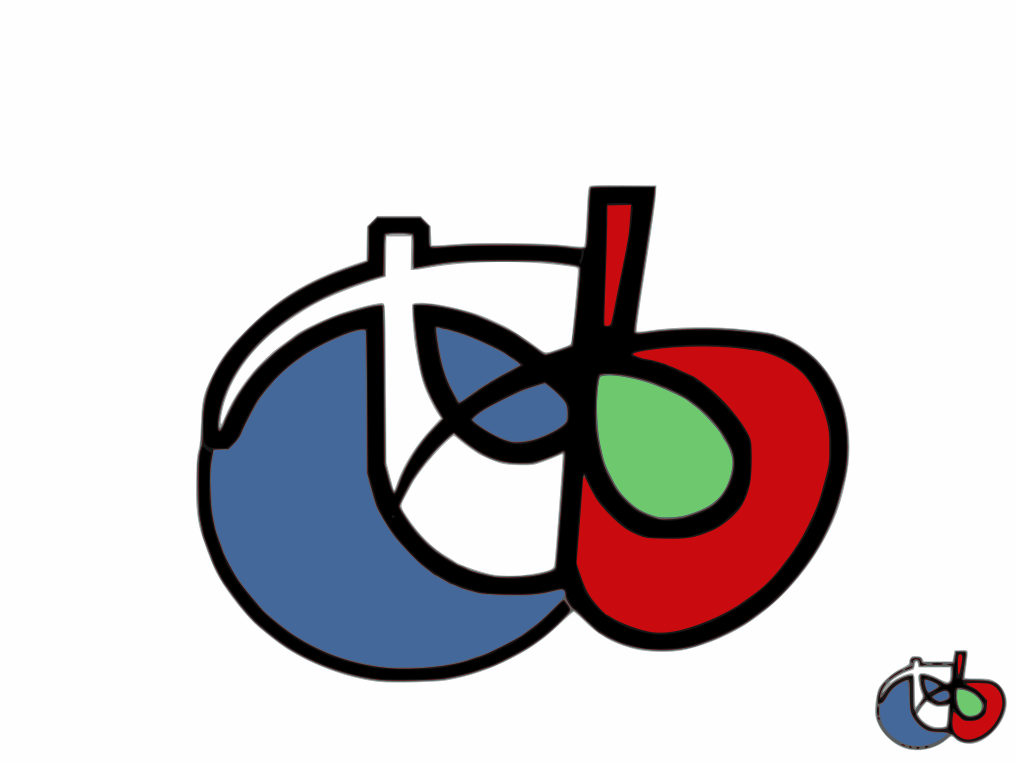
\includegraphics[width=0.2\textwidth]{logoVectoriel}
%% \end{center}
%% \begin{itemize}
%%   \item CNES' free image analysis software
%%    \begin{itemize}
%%      \item Segmentation
%%      \item Feature extraction
%%      \item Registration
%%      \item ...
%%    \end{itemize}
%%   \item Download here \href{http://smsc.cnes.fr/PLEIADES/A_prog_accomp.htm}{http://smsc.cnes.fr/PLEIADES/A\_prog\_accomp.htm}.%{\pgfuseimage{logoIncrust}}.
%% \end{itemize}
%% \end{frame}
\end{document}
